\chapter{Statistical Thermodynamics: Partition Functions}\label{ch:b3:partition-functions}

The tomb of Ludwig Boltzmann in Vienna carries a single line, $S = k\log W$: the
entropy of a system counts the ways its molecules can share out its energy.
Thermodynamics, as the Year 1 and Year 2 volumes built it, never needs
molecules: it relates measured heats, entropies and equilibrium constants to
one another. Statistical thermodynamics computes them from the molecules
themselves. Its central object is a single sum over the energy levels of one
molecule, the partition function; the levels come from spectroscopy, and the
standard entropy of nitrogen computed from its spectrum agrees with the
tabulated value to a hundredth of a joule per kelvin and per mole. This chapter
builds the partition function, splits it into its translational, rotational,
vibrational and electronic parts, and turns it into internal energy, entropy
and Gibbs energy; \cref{ch:b3:statistical-thermo-applied} applies it to heat
capacities and equilibrium constants.

\begin{recall}
The Year 2 volume defined the standard molar entropy, the Gibbs energy and the
chemical potential, and tabulated entropies obtained from heat capacities
measured down to low temperature. \Cref{ch:b3:quantum-model-systems} gave the
energy levels of a \omterm{def:b3:quantum-model-systems:box}{particle in a box}, of the \omterm{def:b3:quantum-model-systems:oscillator}{harmonic oscillator} and of the
\omterm{def:b3:quantum-model-systems:rotor}{rigid rotor}, $E_J = hcBJ(J+1)$ with \omterm{def:b3:quantum-model-systems:degenerate}{degeneracy} $2J + 1$;
\cref{ch:b3:rovibrational-spectroscopy} measured $B$ and $\tilde\nu$ for diatomic
molecules and found that in a homonuclear molecule such as \ce{N2} the
nuclear spins make alternate rotational levels unequal.
\end{recall}

\section{Microstates and the Boltzmann distribution}

Consider $N$ identical, independent molecules that can occupy levels of energy
$\varepsilon_0 = 0 < \varepsilon_1 < \varepsilon_2 < \dots$, with total energy $E$. Saying how many
molecules are on each level, $\{n_0, n_1, \dots\}$, describes a distribution;
saying which molecule is on which level describes much more.

\begin{definition}[Microstate, statistical weight]\label{def:b3:partition-functions:microstate}
A \emph{microstate}\index{microstate} of a system of molecules is a complete
specification of the state of every molecule. The \emph{statistical
weight}\index{statistical weight} $W$ of a distribution $\{n_i\}$ of $N$ molecules over
non-degenerate levels is the number of microstates that realise it:
\[
  W = \frac{N!}{n_0!\,n_1!\,n_2!\cdots}.
\]
\end{definition}

\begin{example}[Three quanta among three oscillators]\label{ex:b3:partition-functions:three-quanta}
Three oscillators share three quanta of energy. The distribution ``one
oscillator holds all three'' can be realised in $3!/(1!\,2!) = 3$ ways, ``one
holds two, another one'' in $3! = 6$ ways and ``each holds one'' in one way:
ten \omterm{def:b3:partition-functions:microstate}{microstates} in all, and the most even distribution that still spreads the
energy over several levels is the most probable. With $10^{23}$ molecules the
weights become so sharply peaked that one distribution, and the ones that differ
from it by a negligible amount, carry practically all the \omterm{def:b3:partition-functions:microstate}{microstates}.
\end{example}

\begin{remark}
The postulate of statistical thermodynamics is that all the \omterm{def:b3:partition-functions:microstate}{microstates} of an
isolated system with a given energy are equally probable. The system is then
found, overwhelmingly, in the distribution of largest weight: finding it is the
task of this section.
\end{remark}

For large numbers, Stirling's approximation $\ln x! \approx x\ln x - x$ gives
\[
  \ln W = N\ln N - \sum_i n_i\ln n_i .
\]

\begin{definition}[Boltzmann distribution, population]\label{def:b3:partition-functions:boltzmann}
The \emph{population}\index{population} $n_i/N$ of a level is the fraction of the
molecules that occupy it. The \emph{Boltzmann distribution}\index{Boltzmann distribution}
is the distribution of largest weight of independent molecules at
thermal equilibrium at temperature $T$, given by the theorem below.
\end{definition}

\begin{theorem}[The Boltzmann distribution]\label{thm:b3:partition-functions:boltzmann}
For independent molecules at equilibrium at temperature $T$, the \omterm{def:b3:partition-functions:boltzmann}{population} of a
level of energy $\varepsilon_i$ and \omterm{def:b3:quantum-model-systems:degenerate}{degeneracy} $g_i$ is
\[
  \frac{n_i}{N} = \frac{g_i\eu^{-\varepsilon_i/kT}}{q},
  \qquad q = \sum_i g_i\eu^{-\varepsilon_i/kT},
\]
where $k$ is the Boltzmann constant. Two levels have \omterm{def:b3:partition-functions:boltzmann}{populations} in the ratio
$\frac{n_j}{n_i} = \frac{g_j}{g_i}\eu^{-(\varepsilon_j - \varepsilon_i)/kT}$.
\end{theorem}

\begin{proof}[Partial proof]
Take first non-degenerate levels. Maximise $\ln W$ under the two constraints
$\sum_in_i = N$ and $\sum_in_i\varepsilon_i = E$ with Lagrange multipliers $\alpha$ and $\beta$:
for every $i$,
\[
  \frac{\partial}{\partial n_i}\Bigl(\ln W + \alpha\sum_jn_j - \beta\sum_jn_j\varepsilon_j\Bigr)
  = -\ln n_i - 1 + \alpha - \beta\varepsilon_i = 0,
\]
so $n_i = \eu^{\alpha - 1}\eu^{-\beta\varepsilon_i}$, and the first constraint fixes $\eu^{\alpha - 1}
= N/\sum_j\eu^{-\beta\varepsilon_j}$. A level of \omterm{def:b3:quantum-model-systems:degenerate}{degeneracy} $g_i$ is $g_i$ distinct states of
the same energy, each populated as above: its \omterm{def:b3:partition-functions:boltzmann}{population} is multiplied by
$g_i$. The multiplier $\beta$ is identified by one known case: for the
translational motion of an ideal gas (\cref{prop:b3:partition-functions:q-trans}
below) the distribution gives an energy $\frac32N/\beta$, and the ideal-gas
energy is $\frac32NkT$; hence $\beta = 1/kT$. That $\beta$ is the same quantity for every
kind of motion, and that it is the thermodynamic temperature, is admitted
here: two systems in thermal contact share the same $\beta$, which is the defining
property of temperature.
\end{proof}

\begin{definition}[Molecular partition function]\label{def:b3:partition-functions:partition-function}
The \emph{molecular partition function}\index{molecular partition function} of a
molecule at temperature $T$ is the sum
\[
  q = \sum_{\text{levels}}g_i\eu^{-\varepsilon_i/kT} = \sum_{\text{states}}\eu^{-\varepsilon_s/kT},
\]
with energies measured from the lowest level, so that $q \ge 1$.
\end{definition}

The partition function counts the states that are thermally accessible: at
very low temperature only the lowest level contributes and $q \to g_0$; at very
high temperature every state contributes about 1 and $q$ grows without limit.
A rule of thumb follows: levels much more than $kT$ above the lowest one are
empty, levels within $kT$ of it are populated. At \qty{298.15}{K}, $kT$ corresponds
to \qty{207.2}{cm^{-1}}, or $RT = \qty{2.479}{kJ/mol}$.

\begin{method}[Populations of levels from spectroscopic constants]\label{met:b3:partition-functions:populations}
\begin{enumerate}
  \item List the levels with their energies (from the constants, e.g.
        $hcBJ(J+1)$) and degeneracies ($2J + 1$).
  \item Express each energy in units of $kT$; at \qty{298.15}{K}, divide a
        wavenumber by \qty{207.2}{cm^{-1}}.
  \item Form the terms $g_i\eu^{-\varepsilon_i/kT}$, add them up to get $q$, and divide.
        Stop the sum when the terms are negligible.
  \item Check: the \omterm{def:b3:partition-functions:boltzmann}{populations} add up to 1; the ratio of two of them is
        $\frac{g_j}{g_i}\eu^{-(\varepsilon_j-\varepsilon_i)/kT}$.
\end{enumerate}
\end{method}

\begin{example}[The rotational levels of hydrogen chloride]\label{ex:b3:partition-functions:hcl}
% ledger: diat:HCl.Be, diat:HCl.ae
For \ce{H^{35}Cl}, $B_0 = B_e - \alpha_e/2 = \qty{10.44}{cm^{-1}}$. At \qty{300}{K} the level $J$
lies at $10.44\,J(J+1)$~\unit{cm^{-1}}, i.e. $0.0501\,J(J+1)$ in units of $kT$. The terms
$(2J+1)\eu^{-0.0501J(J+1)}$ are 1, 2.71, 3.70, 3.84, 3.31, 2.45, \dots; their sum is
$q = 20.3$ and the \omterm{def:b3:partition-functions:boltzmann}{populations} of $J = 0$ to 4 are 0.049, 0.134, 0.182, 0.189 and
0.163: the most populated level is $J = 3$, not $J = 0$, because the \omterm{def:b3:quantum-model-systems:degenerate}{degeneracy}
$2J + 1$ grows while the Boltzmann factor falls. This is the envelope of the
rotation--vibration band of \cref{ch:b3:rovibrational-spectroscopy}.
\end{example}

\begin{omfigure}
\begin{tikzpicture}[font=\small]
  % levels J = 0-3, g = 2J+1, energies 0, 1, 3, 6 (units of 2hcB); bars = 3.5 cm x population
  % of the four levels alone at kT = 2hcB (0.422, 0.466, 0.105, 0.007) and kT = 10hcB (0.120, 0.296, 0.330, 0.254)
  \foreach \J/\e/\g/\lo/\hi in {0/0/1/1.48/0.42, 1/1/3/1.63/1.04, 2/3/5/0.37/1.16, 3/6/7/0.03/0.89}{
    \draw[thick] (0,0.55*\e) -- (2.2,0.55*\e);
    \node[anchor=east] at (0,0.55*\e) {$J = \J$};
    \node[anchor=west, font=\scriptsize] at (2.25,0.55*\e) {$g = \g$};
    \fill[omDef!70] (3.4,0.55*\e-0.11) rectangle ++(\lo,0.22);
    \fill[omThm!70] (6.4,0.55*\e-0.11) rectangle ++(\hi,0.22);
  }
  \node[anchor=south, omDef] at (4.2,3.6) {low $T$};
  \node[anchor=south, omThm] at (7.2,3.6) {high $T$};
  \draw[->] (-1.4,0) -- (-1.4,3.7) node[anchor=south] {$\varepsilon$};
\end{tikzpicture}

{\small A Boltzmann staircase: rotational levels $J = 0$ to 3 (energies $0$, $2$, $6$,
$12$ times $hcB$, degeneracies $2J + 1$) and their \omterm{def:b3:partition-functions:boltzmann}{populations}, as bar lengths,
at $kT = 2hcB$ and $kT = 10hcB$ (the four levels alone). Heating empties the
lowest level towards the upper ones; at both temperatures the bars add up to
the same total, the number of molecules.}
\end{omfigure}

\section{The molecular partition function}

\begin{proposition}[Factorisation]\label{prop:b3:partition-functions:factorisation}
If the energy of a molecule is a sum of independent contributions,
$\varepsilon = \varepsilon^{\mathrm T} + \varepsilon^{\mathrm R} + \varepsilon^{\mathrm V} + \varepsilon^{\mathrm E}$, each state being
any combination of a translational, a rotational, a vibrational and an
electronic state, then
\[
  q = q^{\mathrm T}q^{\mathrm R}q^{\mathrm V}q^{\mathrm E}.
\]
\end{proposition}

\begin{proof}
The sum over all combinations of an exponential of a sum is the product of the
separate sums: $\sum_{a,b}\eu^{-(\varepsilon_a+\varepsilon_b)/kT} = \bigl(\sum_a\eu^{-\varepsilon_a/kT}\bigr)
\bigl(\sum_b\eu^{-\varepsilon_b/kT}\bigr)$, and likewise for four factors.
\end{proof}

The separation is an approximation: rotation and vibration interact (the
constant $\alpha_e$), and the electronic state sets the rotational and vibrational
constants. For a molecule in its ground electronic state at ordinary
temperatures the errors are a few hundredths of a joule per kelvin in an
entropy. The \omterm{def:b3:partition-functions:boltzmann}{populations} are then computed separately for each kind of motion:
the fraction of molecules in a vibrational level $v$ does not depend on their
rotation.

\section{The four contributions}

\subsection*{Translation}

\begin{definition}[Thermal wavelength]\label{def:b3:partition-functions:thermal-wavelength}
The \emph{thermal wavelength}\index{thermal wavelength} of a molecule of mass $m$ at
temperature $T$ is $\Lambda = \dfrac{h}{\sqrt{2\pi mkT}}$.
\end{definition}

\begin{proposition}[Translational partition function]\label{prop:b3:partition-functions:q-trans}
For a molecule of mass $m$ free to move in a volume $V$,
\[
  q^{\mathrm T} = \frac{V}{\Lambda^3}.
\]
\end{proposition}

\begin{proof}
For one dimension, a box of length $L$ has levels $\varepsilon_n = h^2n^2/8mL^2$
($n = 1, 2, \dots$; the zero-point offset changes nothing measurable). They are so
close together that the sum is an integral:
\[
  q_x = \sum_{n\ge1}\eu^{-h^2n^2/8mL^2kT} \approx \int_0^\infty\eu^{-h^2n^2/8mL^2kT}\dd n
      = \frac12\sqrt{\frac{\pi\,8mL^2kT}{h^2}} = \frac{L\sqrt{2\pi mkT}}{h} = \frac{L}{\Lambda}.
\]
The three directions are independent: $q^{\mathrm T} = q_xq_yq_z = L^3/\Lambda^3$. The
mean energy per dimension is $-\partial\ln q_x/\partial\beta$ with $q_x \propto \beta^{-1/2}$, that is
$1/2\beta$; three dimensions give $\frac32kT$ per molecule, as used in the proof of
\cref{thm:b3:partition-functions:boltzmann}.
\end{proof}

\begin{example}[Argon in a flask]\label{ex:b3:partition-functions:argon}
% ledger: aw:Ar, const:h, const:kB
For argon ($M = \qty{39.95}{g/mol}$) at \qty{298.15}{K}, $\Lambda = \qty{16.0}{pm}$, a tenth of an
atomic diameter. In \qty{1}{dm^3}, $q^{\mathrm T} = 10^{-3}/(1.600\times10^{-11})^3 = \num{2.44e29}$
translational states are thermally accessible, far more than the
$2.4\times10^{22}$ atoms the flask holds at \qty{1}{bar}: each state is almost always
empty, the condition under which the molecules can be counted as below.
\end{example}

\subsection*{Rotation}

\begin{definition}[Characteristic temperatures]\label{def:b3:partition-functions:characteristic-temperature}
The \emph{characteristic rotational temperature}\index{characteristic rotational temperature}
of a linear molecule of \omterm{def:b3:rovibrational-spectroscopy:rotational-constant}{rotational constant} $B$ is $\theta_{\mathrm R} =
hcB/k$; the \emph{characteristic vibrational temperature}\index{characteristic vibrational temperature}
of a vibration of wavenumber $\tilde\nu$ is $\theta_{\mathrm V} =
hc\tilde\nu/k$.
\end{definition}

\begin{definition}[Symmetry number]\label{def:b3:partition-functions:symmetry-number}
The \emph{symmetry number}\index{symmetry number} $\sigma$ of a molecule is the
number of distinct orientations of the rigid molecule that are reached by
proper rotations and are indistinguishable from the starting one (the order of
the rotational \omterm{def:b3:point-groups:class}{subgroup} of its \omterm{def:b3:point-groups:point-group}{point group}): 1 for \ce{HCl} and \ce{CO}, 2 for \ce{N2},
\ce{CO2} and \ce{H2O}, 3 for \ce{NH3}, 12 for \ce{CH4} and \ce{C6H6}.
\end{definition}

\begin{proposition}[Rotational partition function]\label{prop:b3:partition-functions:q-rot}
For a linear molecule, $q^{\mathrm R} = \sum_J(2J+1)\eu^{-\theta_{\mathrm R}J(J+1)/T}$. When $T \gg
\theta_{\mathrm R}$,
\[
  q^{\mathrm R} \approx \frac{T}{\sigma\theta_{\mathrm R}} = \frac{kT}{\sigma hcB},
\]
with a relative error of about $\theta_{\mathrm R}/3T$ for $\sigma = 1$ (the exact sum is close
to $T/\theta_{\mathrm R} + \frac13$).
\end{proposition}

\begin{proof}[Partial proof]
For $T \gg \theta_{\mathrm R}$ many levels contribute and the sum becomes an integral.
With $x = J(J+1)$, $\dd x = (2J+1)\dd J$:
\[
  \int_0^\infty(2J+1)\eu^{-\theta_{\mathrm R}J(J+1)/T}\dd J = \int_0^\infty\eu^{-\theta_{\mathrm R}x/T}\dd x
  = \frac{T}{\theta_{\mathrm R}}.
\]
The correction $\frac13$ comes from the next term of the Euler--Maclaurin formula
(\cref{exo:b3:partition-functions:11}). The factor $1/\sigma$ is admitted here and
justified in \cref{ch:b3:statistical-thermo-applied}: in a homonuclear molecule
the symmetry of the wavefunction under the exchange of the two identical nuclei
allows each nuclear-spin state only one parity of $J$
(\cref{ch:b3:rovibrational-spectroscopy}), so on average half the rotational
levels are missing. Counting the rotational states with $\sigma$ in this way
leaves the nuclear-spin states out of $q$; the thermodynamic tables follow the
same convention, and the nuclear-spin factor cancels in every chemical
reaction.
\end{proof}

For \ce{N2}, $B_0 = \qty{1.990}{cm^{-1}}$ and $\theta_{\mathrm R} = \qty{2.86}{K}$: at \qty{298.15}{K},
$q^{\mathrm R} = 298.15/(2\times2.863) = 52.1$. For \ce{HCl}, $\theta_{\mathrm R} = \qty{15.0}{K}$ and
$q^{\mathrm R} = 19.8$ (exact sum 20.2). Only \ce{H2} ($\theta_{\mathrm R} = \qty{85}{K}$) and its \omterm{def:b3:rovibrational-spectroscopy:rotational-constant}{isotopologues}
need the exact sum at room temperature. A non-linear molecule with \omterm{def:b3:rovibrational-spectroscopy:rotational-constant}{rotational
constants} $A$, $B$, $C$ has $q^{\mathrm R} = \frac{1}{\sigma}\bigl(\frac{kT}{hc}\bigr)^{3/2}\sqrt{\frac{\pi}{ABC}}$, admitted.

\subsection*{Vibration}

\begin{proposition}[Vibrational partition function]\label{prop:b3:partition-functions:q-vib}
For a harmonic vibration of wavenumber $\tilde\nu$, with energies measured from the
zero-point level,
\[
  q^{\mathrm V} = \sum_{v\ge0}\eu^{-v\theta_{\mathrm V}/T} = \frac{1}{1 - \eu^{-\theta_{\mathrm V}/T}} .
\]
It tends to 1 when $T \ll \theta_{\mathrm V}$ and to $T/\theta_{\mathrm V}$ when $T \gg \theta_{\mathrm V}$. A molecule
with several \omterm{def:b3:group-theory-applied:normal-mode}{normal modes} has the product of one such factor per mode.
\end{proposition}

\begin{proof}
The levels are $v\,hc\tilde\nu$ above the zero-point level: the sum is a geometric series
of ratio $\eu^{-\theta_{\mathrm V}/T} < 1$. When $T \gg \theta_{\mathrm V}$, $1 - \eu^{-\theta_{\mathrm V}/T} \approx \theta_{\mathrm V}/T$.
The \omterm{def:b3:group-theory-applied:normal-mode}{normal modes} are independent (\cref{prop:b3:partition-functions:factorisation}).
\end{proof}

For the vibrational quantum of a diatomic molecule this book takes the
observed fundamental $G(1) - G(0) = \omega_e - 2\omega_ex_e$
(\cref{ch:b3:rovibrational-spectroscopy}); at room temperature only the first
levels matter, and their spacing is what counts. Stiff, light molecules are
frozen: \ce{N2} has $\theta_{\mathrm V} = \qty{3352}{K}$, $q^{\mathrm V} = 1.000013$ at \qty{298.15}{K}, and
only 13 molecules in a million are in $v = 1$. Heavy, soft ones are not: \ce{I2}
has $\theta_{\mathrm V} = \qty{307}{K}$, $q^{\mathrm V} = 1.556$, and more than a third of its molecules
vibrate.

\begin{omfigure}
\begin{tikzpicture}
\begin{axis}[name=rotA, width=0.36\linewidth, height=5.0cm, xmin=-0.5, xmax=14.5,
  ymin=0, ymax=0.34, axis lines=left, ycomb, xlabel={$J$}, ylabel={population},
  tick label style={font=\scriptsize}, label style={font=\small},
  title={\small \ce{HCl}, rotation}, scaled y ticks=false,
  yticklabel style={/pgf/number format/fixed}]
\addplot[omDef, line width=1.6pt, xshift=-1.6pt] table[x=J, y=T100] {figdata/out/bachelor-3-boltzmann-populations-hcl.dat};
\addplot[black!60, line width=1.6pt] table[x=J, y=T300] {figdata/out/bachelor-3-boltzmann-populations-hcl.dat};
\addplot[omThm, line width=1.6pt, xshift=1.6pt] table[x=J, y=T1000] {figdata/out/bachelor-3-boltzmann-populations-hcl.dat};
\end{axis}
\begin{axis}[name=rotB, at={(rotA.east)}, anchor=west, xshift=0.9cm, width=0.36\linewidth,
  height=5.0cm, xmin=-1, xmax=41, ymin=0, ymax=0.17, axis lines=left, ycomb,
  xlabel={$J$}, tick label style={font=\scriptsize}, label style={font=\small},
  title={\small \ce{CO}, rotation}, scaled y ticks=false,
  yticklabel style={/pgf/number format/fixed}]
\addplot[omDef, sharp plot, thin, mark=*, mark size=0.9pt] table[x=J, y=T100] {figdata/out/bachelor-3-boltzmann-populations-co.dat};
\addplot[black!60, sharp plot, thin, mark=*, mark size=0.9pt] table[x=J, y=T300] {figdata/out/bachelor-3-boltzmann-populations-co.dat};
\addplot[omThm, sharp plot, thin, mark=*, mark size=0.9pt] table[x=J, y=T1000] {figdata/out/bachelor-3-boltzmann-populations-co.dat};
\end{axis}
\begin{axis}[at={(rotB.east)}, anchor=west, xshift=0.9cm, width=0.32\linewidth,
  height=5.0cm, xmin=-0.5, xmax=10.5, ymin=0, ymax=0.7, axis lines=left, ycomb,
  xlabel={$v$}, tick label style={font=\scriptsize}, label style={font=\small},
  title={\small \ce{I2}, vibration}, scaled y ticks=false,
  yticklabel style={/pgf/number format/fixed}]
\addplot[black!60, line width=1.6pt, xshift=-1.2pt] table[x=v, y=T300] {figdata/out/bachelor-3-boltzmann-populations-i2.dat};
\addplot[omThm, line width=1.6pt, xshift=1.2pt] table[x=v, y=T1000] {figdata/out/bachelor-3-boltzmann-populations-i2.dat};
\end{axis}
\end{tikzpicture}

{\small Boltzmann \omterm{def:b3:partition-functions:boltzmann}{populations} computed from the spectroscopic constants:
rotational levels of \ce{H^{35}Cl} ($\theta_{\mathrm R} = \qty{15.0}{K}$) and of \ce{CO}
($\theta_{\mathrm R} = \qty{2.77}{K}$; points joined for legibility) at \qty{100}{K} (blue), \qty{300}{K} (grey) and \qty{1000}{K} (red), and
vibrational levels of \ce{I2} ($\theta_{\mathrm V} = \qty{307}{K}$) at 300 and \qty{1000}{K}. Rotational
\omterm{def:b3:partition-functions:boltzmann}{populations} peak at $J > 0$; vibrational ones always decrease with $v$, since
the levels are not degenerate.}
\end{omfigure}

\subsection*{Electronic states}

\begin{proposition}[Electronic partition function]\label{prop:b3:partition-functions:q-elec}
With the electronic levels $\varepsilon_j$ (\omterm{def:b3:quantum-model-systems:degenerate}{degeneracy} $g_j$) measured from the ground
level,
\[
  q^{\mathrm E} = g_0 + g_1\eu^{-\varepsilon_1/kT} + \cdots
\]
For most molecules the first excited electronic level lies tens of thousands of
wavenumbers up and $q^{\mathrm E} = g_0$: 1 for a closed-shell molecule, 3 for
\ce{O2} (ground term ${}^3\Sigma_g^-$), $2J + 1$ for an atom in a level $J$.
\end{proposition}

This is the definition applied to the electronic levels; the cases where low
levels matter are atoms and radicals with a \omterm{def:b3:many-electron-atoms:spin-orbit}{fine structure}.

\begin{example}[Nitric oxide and the chlorine atom]\label{ex:b3:partition-functions:no-cl}
% ledger: diat:NO.split, lev:Cl.2P1_2
\ce{NO} has a ${}^2\Pi$ ground term split by \omterm{def:b3:many-electron-atoms:spin-orbit}{spin--orbit coupling} into ${}^2\Pi_{1/2}$ (lower)
and ${}^2\Pi_{3/2}$, \qty{119.73}{cm^{-1}} higher, each doubly degenerate. At \qty{298.15}{K},
$q^{\mathrm E} = 2 + 2\eu^{-119.73/207.22} = 2 + 2\times0.561 = 3.12$: 36\,\% of the molecules are in
the upper component. The chlorine atom has its ${}^2P_{1/2}$ level \qty{882.35}{cm^{-1}}
above the ${}^2P_{3/2}$ ground level: $q^{\mathrm E} = 4 + 2\eu^{-4.258} = 4.03$.
\end{example}

\begin{omfigure}
\begin{tikzpicture}
\begin{axis}[name=qr, width=0.48\linewidth, height=5.4cm, xmin=0, xmax=300, ymin=0,
  ymax=22, axis lines=left, xlabel={$T$ / K}, ylabel={$q^{\mathrm R}$},
  tick label style={font=\scriptsize}, label style={font=\small},
  title={\small rotation of \ce{HCl}}, legend style={font=\scriptsize, draw=none,
  fill=white, fill opacity=0.85, text opacity=1, at={(0.03,0.97)}, anchor=north west},
  legend cell align=left]
\addplot[black, thick] table[x=T, y=exact] {figdata/out/bachelor-3-partition-functions-rot.dat};
\addplot[omDef, thick, dashed] table[x=T, y=high] {figdata/out/bachelor-3-partition-functions-rot.dat};
\addplot[omThm, thin, densely dotted] table[x=T, y=corr] {figdata/out/bachelor-3-partition-functions-rot.dat};
\legend{exact sum, $T/\theta_{\mathrm R}$, $T/\theta_{\mathrm R} + \frac13$}
\end{axis}
\begin{axis}[at={(qr.east)}, anchor=west, xshift=1.3cm, width=0.48\linewidth, height=5.4cm,
  xmin=0, xmax=3000, ymin=0.8, ymax=11, axis lines=left, xlabel={$T$ / K},
  ylabel={$q^{\mathrm V}$}, tick label style={font=\scriptsize},
  label style={font=\small}, title={\small vibration},
  scaled x ticks=false, xticklabel style={/pgf/number format/1000 sep={}}]
\addplot[omDef, thick] table[x=T, y=N2] {figdata/out/bachelor-3-partition-functions-vib.dat};
\addplot[black!60, thick] table[x=T, y=Cl2] {figdata/out/bachelor-3-partition-functions-vib.dat};
\addplot[omThm, thick] table[x=T, y=I2] {figdata/out/bachelor-3-partition-functions-vib.dat};
\node[font=\scriptsize, omThm, anchor=south east] at (axis cs:2700,9.3) {\ce{I2} (\qty{307}{K})};
\node[font=\scriptsize, black!70, anchor=south east] at (axis cs:2950,4.45) {\ce{Cl2} (\qty{798}{K})};
\node[font=\scriptsize, omDef, anchor=south east] at (axis cs:2950,1.55) {\ce{N2} (\qty{3352}{K})};
\end{axis}
\end{tikzpicture}

{\small Left: the rotational partition function of \ce{HCl} ($\theta_{\mathrm R} = \qty{15.0}{K}$),
exact sum against the high-temperature form; the form with the correction
$\frac13$ is indistinguishable from the sum above about \qty{30}{K}. Right: the vibrational
partition function of three diatomic molecules (characteristic temperatures in
brackets), 1 while $T \ll \theta_{\mathrm V}$, then close to $T/\theta_{\mathrm V}$.}
\end{omfigure}

\section{From partition functions to thermodynamics}

\begin{theorem}[Internal energy]\label{thm:b3:partition-functions:internal-energy}
For $N$ independent molecules, the internal energy measured from its value at
$T = 0$ is
\[
  U - U(0) = NkT^2\Bigl(\frac{\partial\ln q}{\partial T}\Bigr)_V
          = -N\Bigl(\frac{\partial\ln q}{\partial\beta}\Bigr)_V .
\]
The contributions of the four kinds of motion add up.
\end{theorem}

\begin{proof}
$U - U(0) = \sum_in_i\varepsilon_i = \frac Nq\sum_ig_i\varepsilon_i\eu^{-\beta\varepsilon_i} = -\frac Nq\frac{\partial q}{\partial\beta}$;
and $\dd\beta = -\dd T/kT^2$. The volume is held fixed because the translational
levels depend on it. By \cref{prop:b3:partition-functions:factorisation}, $\ln q$ is a
sum of four terms.
\end{proof}

For translation, $q^{\mathrm T} \propto T^{3/2}$ gives $\frac32NkT$; for the rotation of a linear
molecule at high temperature, $q^{\mathrm R} \propto T$ gives $NkT$; a vibration gives
$Nk\theta_{\mathrm V}/(\eu^{\theta_{\mathrm V}/T} - 1)$, which is $NkT$ only when $T \gg \theta_{\mathrm V}$. The
classical equipartition of energy, $\frac12kT$ per quadratic term, is the
high-temperature limit of these results; \cref{ch:b3:statistical-thermo-applied}
follows the heat capacities as each motion freezes out.

\begin{definition}[Canonical partition function]\label{def:b3:partition-functions:canonical}
The \emph{canonical partition function}\index{canonical partition function} of a
system at temperature $T$ and volume $V$ is the sum $Q = \sum_s\eu^{-E_s/kT}$ over all the
states $s$ of the whole system, of energies $E_s$.
\end{definition}

\begin{proposition}[Canonical partition function of an ideal gas]\label{prop:b3:partition-functions:canonical}
For $N$ independent molecules, $Q = q^N$ if they are distinguishable (localised in
a crystal), and $Q = q^N/N!$ for an ideal gas of identical molecules.
\end{proposition}

\begin{proof}[Partial proof]
A state of the system is a choice of state for each molecule and the energies
add up: the sum of the products is the product of the sums, $q^N$. In a gas the
molecules are \omterm{def:b3:many-electron-atoms:indistinguishable}{indistinguishable}: permuting them gives the same state of the
system. When the molecular states are far more numerous than the molecules
(\cref{ex:b3:partition-functions:argon}), almost every term of $q^N$ has its $N$
molecules in different states and is counted $N!$ times. Cases where two
molecules share a state, which this counting gets wrong, are negligible except
at very low temperature or very high density, where quantum statistics take
over (admitted).
\end{proof}

\begin{definition}[Statistical entropy]\label{def:b3:partition-functions:statistical-entropy}
The \emph{statistical entropy}\index{statistical entropy} of an isolated system is
$S = k\ln W$, where $W$ is the number of its \omterm{def:b3:partition-functions:microstate}{microstates}; for a system at
temperature $T$, $W$ is the weight of the dominant distribution.
\end{definition}

\begin{theorem}[Entropy and the other functions]\label{thm:b3:partition-functions:entropy}
For a system at temperature $T$ with \omterm{def:b3:partition-functions:canonical}{canonical partition function} $Q$,
\[
  S = \frac{U - U(0)}{T} + k\ln Q, \qquad A - A(0) = -kT\ln Q, \qquad
  p = kT\Bigl(\frac{\partial\ln Q}{\partial V}\Bigr)_T .
\]
For an ideal gas this gives $pV = NkT$ and $G - G(0) = -NkT\ln(q/N)$.
\end{theorem}

\begin{proof}[Partial proof]
For distinguishable molecules in the \omterm{def:b3:partition-functions:boltzmann}{Boltzmann distribution}, with $n_i = Ng_i\eu^{-\beta\varepsilon_i}/q$
and Stirling's formula, the weight $W = N!\prod_ig_i^{n_i}/n_i!$ gives
\[
  \ln W = N\ln N - \sum_in_i\ln\frac{n_i}{g_i} = N\ln N - \sum_in_i\Bigl(\ln\frac Nq - \beta\varepsilon_i\Bigr)
        = N\ln q + \beta\,(U - U(0)),
\]
so $k\ln W = k\ln q^N + (U - U(0))/T$; for a gas, $q^N$ becomes $q^N/N!$. The
identification of $k\ln W$ with the thermodynamic entropy is admitted: it is
additive, maximal at equilibrium for an isolated system, and gives back the
ideal-gas relations. Then $A = U - TS$ gives the second formula, $p =
-(\partial A/\partial V)_T$ the third: with $Q = q^N/N!$ and $q \propto V$, $p = NkT/V$. Finally
$G = A + pV = -kT\ln(q^N/N!) + NkT = -NkT\ln(q/N)$, using $\ln N! = N\ln N - N$.
\end{proof}

\begin{theorem}[Sackur--Tetrode equation]\label{thm:b3:partition-functions:sackur-tetrode}
The molar entropy of a monatomic ideal gas of molar mass $M$ at temperature $T$
and pressure $p$ is
\[
  S_{\mathrm m} = R\Bigl[\ln\Bigl(\frac{kT}{p\Lambda^3}\Bigr) + \frac52\Bigr],
  \qquad \Lambda = \frac{h}{\sqrt{2\pi mkT}},\ m = \frac{M}{N_A}.
\]
\end{theorem}

\begin{proof}
With $Q = q^N/N!$, $q = V/\Lambda^3$ and $U - U(0) = \frac32NkT$,
\cref{thm:b3:partition-functions:entropy} gives $S = \frac32Nk + Nk\ln q - k(N\ln N - N) =
Nk\bigl[\ln\frac{V}{N\Lambda^3} + \frac52\bigr]$. For one mole, $Nk = R$ and $V/N = kT/p$.
\end{proof}

For argon at \qty{298.15}{K} and \qty{1}{bar}, $kT/p = \qty{4.116e-26}{m^3}$ and $\Lambda =
\qty{1.600e-11}{m}$: $S_{\mathrm m} = R(\ln\num{1.005e7} + 2.5) = \qty{154.85}{J.K^{-1}.mol^{-1}}$. The
tabulated standard entropy, obtained from heat capacities measured down to a
few kelvins, is $154.846 \pm 0.003$: the formula has no adjustable parameter, and
it contains Planck's constant. A heavier atom has a larger entropy (more
translational states at the same energy), and so has a gas at lower pressure
(more volume per atom).

\begin{proposition}[Rotational and vibrational molar entropies]\label{prop:b3:partition-functions:modes-entropy}
For a linear molecule with $T \gg \theta_{\mathrm R}$, and a vibration with $x = \theta_{\mathrm V}/T$,
\[
  S^{\mathrm R}_{\mathrm m} = R\Bigl[\ln\frac{T}{\sigma\theta_{\mathrm R}} + 1\Bigr],
  \qquad
  S^{\mathrm V}_{\mathrm m} = R\Bigl[\frac{x}{\eu^x - 1} - \ln\bigl(1 - \eu^{-x}\bigr)\Bigr],
\]
and an electronic ground level of \omterm{def:b3:quantum-model-systems:degenerate}{degeneracy} $g_0$, alone populated, adds $R\ln g_0$.
\end{proposition}

\begin{proof}
For internal motions the factor $1/N!$ belongs to translation only, so each
internal mode contributes $S = \frac{U - U(0)}{T} + Nk\ln q$. Rotation:
$q = T/\sigma\theta_{\mathrm R}$ and $U - U(0) = NkT$. Vibration: $\ln q = -\ln(1 - \eu^{-x})$ and
$(U - U(0))/T = Nkx/(\eu^x - 1)$. Electronic: $q = g_0$, $U - U(0) = 0$.
\end{proof}

\begin{method}[The standard entropy of a gas from its constants]\label{met:b3:partition-functions:standard-entropy}
\begin{enumerate}
  \item Translation: Sackur--Tetrode with the molar mass, $T = \qty{298.15}{K}$ and
        $p^\circ = \qty{1}{bar}$.
  \item Rotation: $B_0 = B_e - \alpha_e/2$, $\theta_{\mathrm R} = hcB_0/k$, the \omterm{def:b3:partition-functions:symmetry-number}{symmetry number},
        and $R[\ln(T/\sigma\theta_{\mathrm R}) + 1]$ (or the exact sum if $T < 30\,\theta_{\mathrm R}$).
  \item Vibration: one term per \omterm{def:b3:group-theory-applied:normal-mode}{normal mode}, with the fundamental wavenumbers.
  \item Electronic: $R\ln g_0$, or $R[\ln q^{\mathrm E} + \langle\varepsilon\rangle/kT]$ if low levels exist.
  \item Add; compare with the table, where nuclear spin is left out in the same way.
\end{enumerate}
\end{method}

\begin{center}\small
% table: sackur-tetrode (checked by tests/bachelor-3/test_sackur-tetrode.py)
% ledger: s0:Ar_g, s0:N2_g, s0:CO_g, s0:HCl_g, s0:Cl2_g, s0:I2_g, s0:Cl_g
\begin{tabular}{lrrrrrr}
\hline
gas & $S^{\mathrm T}$ & $S^{\mathrm R}$ & $S^{\mathrm V}$ & $S^{\mathrm E}$ & sum & table \\ \hline
\ce{Ar} & 154.85 & 0.00 & 0.00 & 0.00 & 154.85 & 154.85 \\
\ce{N2} & 150.42 & 41.18 & 0.00 & 0.00 & 191.60 & 191.61 \\
\ce{CO} & 150.42 & 47.23 & 0.00 & 0.00 & 197.65 & 197.66 \\
\ce{HCl} & 153.71 & 33.16 & 0.00 & 0.00 & 186.87 & 186.90 \\
\ce{Cl2} & 162.00 & 58.65 & 2.24 & 0.00 & 222.89 & 223.08 \\
\ce{I2} & 177.91 & 74.24 & 8.43 & 0.00 & 260.58 & 260.69 \\
\ce{Cl} & 153.36 & 0.00 & 0.00 & 11.83 & 165.19 & 165.19 \\ \hline
\end{tabular}

\smallskip
Statistical standard molar entropies at \qty{298.15}{K} and \qty{1}{bar}, in
\unit{J.K^{-1}.mol^{-1}}, from the spectroscopic constants, against the tabulated values.
\end{center}

The sums agree with the tables to better than 0.2 \unit{J.K^{-1}.mol^{-1}}, and to a few
hundredths for the light molecules. The small residuals of \ce{Cl2} and \ce{I2} come
from approximations this chapter made: the constants of the main \omterm{def:b3:rovibrational-spectroscopy:rotational-constant}{isotopologue},
the \omterm{def:b3:quantum-model-systems:oscillator}{harmonic oscillator} for a molecule with many vibrational levels
populated. The tabulated entropy of \ce{CO} is itself the statistical value:
measured calorimetrically, it comes out several \unit{J.K^{-1}.mol^{-1}} lower, a discrepancy
explained in \cref{ch:b3:statistical-thermo-applied}.

\begin{inthelab}[Measuring a third-law entropy]
The calorimetric route heats a sample from a few kelvins to \qty{298.15}{K} in an
adiabatic calorimeter, measuring its heat capacity in small steps. The
entropy is the sum of $\int C_p\dd T/T$ over each phase, plus $\Delta H/T$ at every
transition (solid--solid, fusion, vaporisation), plus a small correction for
the non-ideality of the real gas; below the lowest measured temperature,
$C_p$ of a non-metallic solid is extrapolated as $aT^3$. The third law fixes the
entropy of the perfect crystal at 0 K to zero. Agreement with the statistical
value, within the uncertainty of the measurement, both tests the third law and
reveals the crystals that are not perfect at 0 K.
\end{inthelab}

\begin{history}[Boltzmann, 1877]
\begin{minipage}[t]{0.72\linewidth}
Ludwig Boltzmann showed in 1877 that the entropy of a gas is proportional to
the logarithm of the number of ways its molecules can share the energy, and
derived the distribution that bears his name by counting those ways. The
interpretation was fiercely contested by physicists who doubted the existence
of atoms. The formula in the form $S = k\log W$, with the constant $k$, was
written by Max Planck, who used the same counting in 1900 for the radiation of
a hot body; it is carved on Boltzmann's tomb in the central cemetery of
Vienna.
\end{minipage}\hfill
\begin{minipage}[t]{0.22\linewidth}\vspace{0pt}
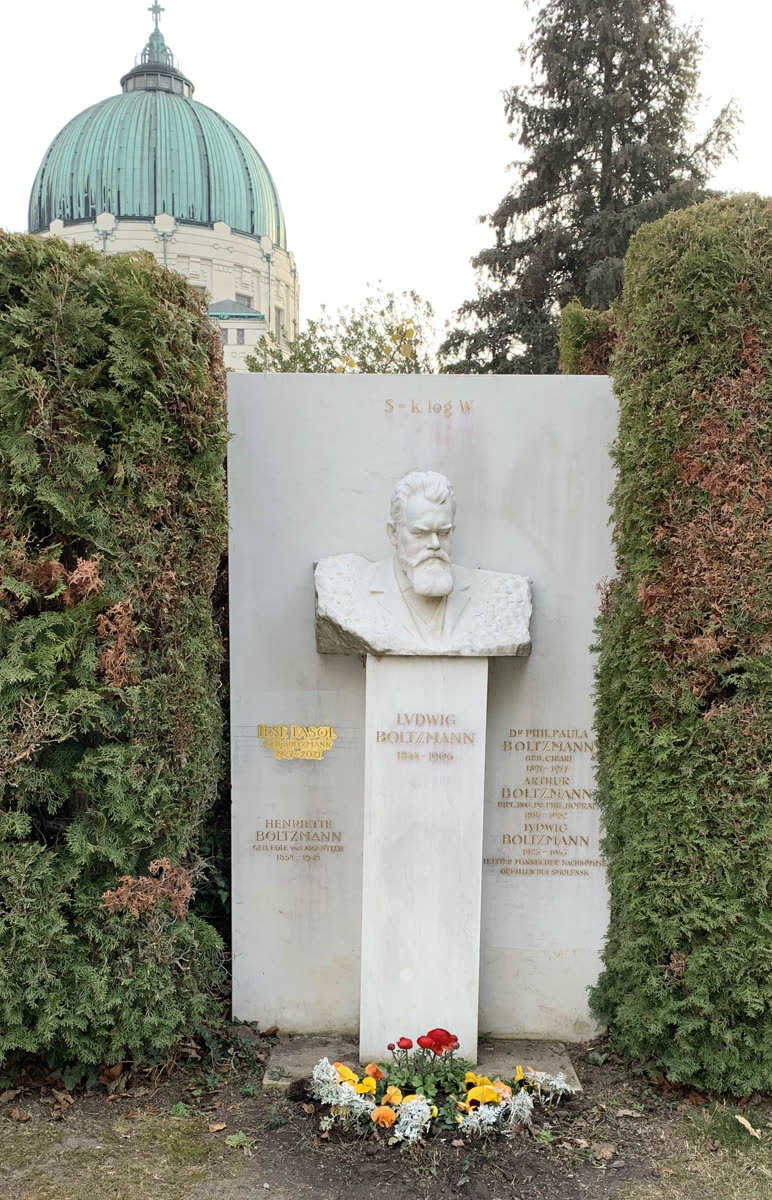
\includegraphics[width=\linewidth]{images/book4/boltzmann-grave.jpg}\par
{\footnotesize The tomb of Boltzmann.}
\end{minipage}
\end{history}

\section{Exercises}

\begin{exercise}[$\star$]\label{exo:b3:partition-functions:1}
Four oscillators share four quanta. List the distributions, give the weight of
each, and check that they add up to the number of ways of placing four
\omterm{def:b3:many-electron-atoms:indistinguishable}{indistinguishable} quanta in four oscillators, $\binom{7}{3}$. Which distributions are the
most probable?
\end{exercise}

\begin{exercise}[$\star$]\label{exo:b3:partition-functions:2}
Two non-degenerate levels are \qty{2.5}{kJ/mol} apart. Compute the ratio of their
\omterm{def:b3:partition-functions:boltzmann}{populations} at \qty{298.15}{K} and at \qty{1000}{K}. What is the limit at very high
temperature?
\end{exercise}

\begin{exercise}[$\star$]\label{exo:b3:partition-functions:3}
% ledger: aw:Ar
Compute the \omterm{def:b3:partition-functions:thermal-wavelength}{thermal wavelength} of an argon atom at \qty{298.15}{K} and its
translational partition function in a volume of \qty{1}{dm^3}.
\end{exercise}

\begin{exercise}[$\star$]\label{exo:b3:partition-functions:4}
% ledger: diat:N2.Be, diat:N2.ae, diat:HCl.Be, diat:HCl.ae
With $B_0 = \qty{1.990}{cm^{-1}}$ (\ce{N2}) and \qty{10.440}{cm^{-1}} (\ce{H^{35}Cl}), compute $\theta_{\mathrm R}$ and the
high-temperature rotational partition function of each molecule at
\qty{298.15}{K}.
\end{exercise}

\begin{exercise}[$\star\star$]\label{exo:b3:partition-functions:5}
% ledger: diat:I2.we, diat:I2.wexe, diat:N2.we, diat:N2.wexe
The fundamental wavenumbers of \ce{I2} and \ce{N2} are \qty{213.27}{cm^{-1}} and
\qty{2329.92}{cm^{-1}}. Compute $\theta_{\mathrm V}$, $q^{\mathrm V}$ at \qty{298.15}{K}, and the fraction of molecules
that are not in $v = 0$.
\end{exercise}

\begin{exercise}[$\star\star$]\label{exo:b3:partition-functions:6}
% ledger: diat:NO.split, lev:Cl.2P1_2
Compute the electronic partition function at \qty{298.15}{K} of \ce{NO} (two doubly
\omterm{def:b3:quantum-model-systems:degenerate}{degenerate levels} \qty{119.73}{cm^{-1}} apart) and of the chlorine atom (${}^2P_{3/2}$
ground level, ${}^2P_{1/2}$ at \qty{882.35}{cm^{-1}}). Which fraction of the \ce{NO} molecules is in
the upper level? What does $q^{\mathrm E}(\ce{NO})$ tend to at high temperature?
\end{exercise}

\begin{exercise}[$\star\star$]\label{exo:b3:partition-functions:7}
From $q^{\mathrm T} = V/\Lambda^3$, derive the internal energy and the heat capacity at
constant volume of one mole of a monatomic ideal gas, and evaluate $U - U(0)$ at
\qty{298.15}{K}.
\end{exercise}

\begin{exercise}[$\star\star$]\label{exo:b3:partition-functions:8}
% ledger: aw:Ar, s0:Ar_g
Use the Sackur--Tetrode equation to compute the standard molar entropy of
argon at \qty{298.15}{K}; compare with the tabulated
\qty{154.846}{J.K^{-1}.mol^{-1}}. By how much does it change if the pressure is divided by 10?
\end{exercise}

\begin{exercise}[$\star\star$]\label{exo:b3:partition-functions:9}
% ledger: diat:HCl.Be, diat:HCl.ae
Compute the rotational contribution to the standard molar entropy of
\ce{H^{35}Cl} at \qty{298.15}{K} ($\theta_{\mathrm R} = \qty{15.02}{K}$).
\end{exercise}

\begin{exercise}[$\star\star\star$]\label{exo:b3:partition-functions:10}
Treating $J$ as continuous, show that the most populated rotational level of a
linear molecule is near $J_{\max} = \sqrt{T/2\theta_{\mathrm R}} - \frac12$. Evaluate it for \ce{HCl}
($\theta_{\mathrm R} = \qty{15.02}{K}$) and \ce{CO} ($\theta_{\mathrm R} = \qty{2.766}{K}$) at \qty{300}{K}. Why are the two
branches of an infrared band strongest a few lines away from the centre?
\end{exercise}

\begin{exercise}[$\star\star\star$]\label{exo:b3:partition-functions:11}
% ledger: diat:H2.Be, diat:H2.ae
The Euler--Maclaurin formula gives $\sum_{J\ge0}f(J) \approx \int_0^\infty f(J)\dd J + \frac12f(0) -
\frac1{12}f'(0)$. Apply it to $f(J) = (2J+1)\eu^{-\theta J(J+1)/T}$ and show that $q^{\mathrm R} \approx T/\theta +
\frac13$. For which temperatures is $T/\theta$ correct to 1\,\%? Is it acceptable for \ce{H2}
($B_0 = \qty{59.32}{cm^{-1}}$) at \qty{298.15}{K}?
\end{exercise}

\begin{exercise}[$\star\star\star$]\label{exo:b3:partition-functions:12}
% ledger: diat:I2.we, diat:I2.wexe
Show that the vibrational molar entropy tends to zero when $T \ll \theta_{\mathrm V}$ and to
$R[1 + \ln(T/\theta_{\mathrm V})]$ when $T \gg \theta_{\mathrm V}$. Evaluate both the exact expression and this
limit for \ce{I2} ($\theta_{\mathrm V} = \qty{306.9}{K}$) at \qty{298.15}{K}, and comment.
\end{exercise}

\section{Problem: Counting the Entropy of Nitrogen}

\begin{problem}[{Weekend problem --- counting the entropy of nitrogen: the
translational, rotational, vibrational and electronic contributions to its
standard entropy, computed from its spectrum and compared with the table}]
\label{pb:b3:partition-functions:1}
% ledger: aw:N, diat:N2.Be, diat:N2.ae, diat:N2.we, diat:N2.wexe, s0:N2_g, const:h, const:kB, const:NA, const:c
Nitrogen is the main gas of the air. Its standard molar entropy at
\qty{298.15}{K} is computed here from its molar mass, \qty{28.014}{g/mol}, and from its
spectroscopic constants: $B_e = \qty{1.998241}{cm^{-1}}$, $\alpha_e = \qty{0.017318}{cm^{-1}}$, $\omega_e =
\qty{2358.57}{cm^{-1}}$, $\omega_ex_e = \qty{14.324}{cm^{-1}}$; its electronic ground term is ${}^1\Sigma_g^+$.
Standard pressure $p^\circ = \qty{1}{bar}$; $k = \qty{1.380649e-23}{J/K}$, $h = \qty{6.62607015e-34}{J.s}$.

\medskip\noindent\textbf{Part I --- Translation.}
\begin{enumerate}
  \item Compute the mass of one molecule.
  \item Compute its \omterm{def:b3:partition-functions:thermal-wavelength}{thermal wavelength} at \qty{298.15}{K}.
  \item Compute the volume available per molecule, $kT/p^\circ$.
  \item Deduce $q^{\mathrm T}/N$, and comment on its size.
  \item Compute the translational molar entropy.
  \item By how much would it change at half the pressure?
\end{enumerate}

\medskip\noindent\textbf{Part II --- Rotation.}
\begin{enumerate}[resume]
  \item Compute $B_0$.
  \item Compute $\theta_{\mathrm R}$.
  \item Give the \omterm{def:b3:partition-functions:symmetry-number}{symmetry number} and say what it accounts for.
  \item Compute $q^{\mathrm R}$ at \qty{298.15}{K}.
  \item Is the high-temperature form justified?
  \item Compute the rotational molar entropy.
  \item Ignoring the nuclear-spin weights, which rotational level is the most
        populated?
\end{enumerate}

\medskip\noindent\textbf{Part III --- Vibration and electronic states.}
\begin{enumerate}[resume]
  \item Compute the vibrational quantum $G(1) - G(0)$.
  \item Compute $\theta_{\mathrm V}$.
  \item Compute $q^{\mathrm V}$ at \qty{298.15}{K}.
  \item What fraction of the molecules is in $v = 1$?
  \item Compute the vibrational molar entropy.
  \item What is the electronic contribution? Why can excited electronic states
        be ignored?
\end{enumerate}

\medskip\noindent\textbf{Part IV --- Sum and comparison.}
\begin{enumerate}[resume]
  \item Add the contributions.
  \item Compare with the tabulated \qty{191.609}{J.K^{-1}.mol^{-1}}.
  \item Which measurements does the calorimetric value of a table rest on?
  \item Why can the tables leave nuclear spin out?
  \item State the result: the standard molar entropy of nitrogen at \qty{298.15}{K}
        computed from its spectroscopic constants.
\end{enumerate}
\end{problem}
